\documentclass[12pt, A4]{article}
\usepackage[utf8]{inputenc}
\usepackage{graphicx}
\usepackage[margin=0.5in]{geometry}
\usepackage{hyperref}
\usepackage{datetime}

\title{Lab 1 Report}
\author{Anton Gashi: 201914462 \\ Email: \href{anton.gashi.2019@uni.strath.ac.uk}{anton.gashi.2019@uni.strath.ac.uk} \\ Github: \href{https://github.com/AntonGashi/Computation_Class}{/Lab1/}}
\date{\today}

\begin{document}
\begin{titlepage}
\clearpage\maketitle
\thispagestyle{empty}
\end{titlepage}


\section*{\underline{Task 1}}
\textbf{Task From Lab Sheet:} \\ \\ Using different initial seeds and at least two different pseudo-random generators, produce sequences of uniformly distributed random numbers. Test these values for a) uniformity and b) lack of sequential correlation. Present your analysis as graphically as possible.
\vspace{1.5em}\\
\textbf{My Result:} \\ \\ The two different pseudo-random generators I used were \href{https://numpy.org/doc/stable/reference/random/generated/numpy.random.uniform.html}{numpy.random.uniform} and \href{https://numpy.org/doc/stable/reference/random/generated/numpy.random.choice.html}{numpy.random.choice}. \\ The Chi squared for the uniform distribution is $\chi_{uniform}$ = 89.42 ($\le$ 100) and $\chi_{choice}$ = 158.36 for the random choice distribution, the reason for the larger Chi squared value for the second generator is due to the fact that the choice is made from the first generator \textbf{with} replacement. If 'replace=False' then the Chi squared becomes the exact same as the first. I also used the \href{"https://numpy.org/doc/stable/reference/generated/numpy.corrcoef.html"}{np.corrcoef} function which returns a Pearson product-moment correlation, this gives an array with either diagonal representing the correlation between each array from -1 to 1, -1 being a negative 45 degree gradient and 1 being a positive 45 degree gradient. This correlation only accounts for linear correlations, so say the data looked sinusoidal in figure \ref{fig1} then the correlation would still be 0. Furthermore from inspection of the two figures\ref{fig1} bellow, using different seeds, there seems to be no correlation.

\begin{figure}[h]
  \centering
    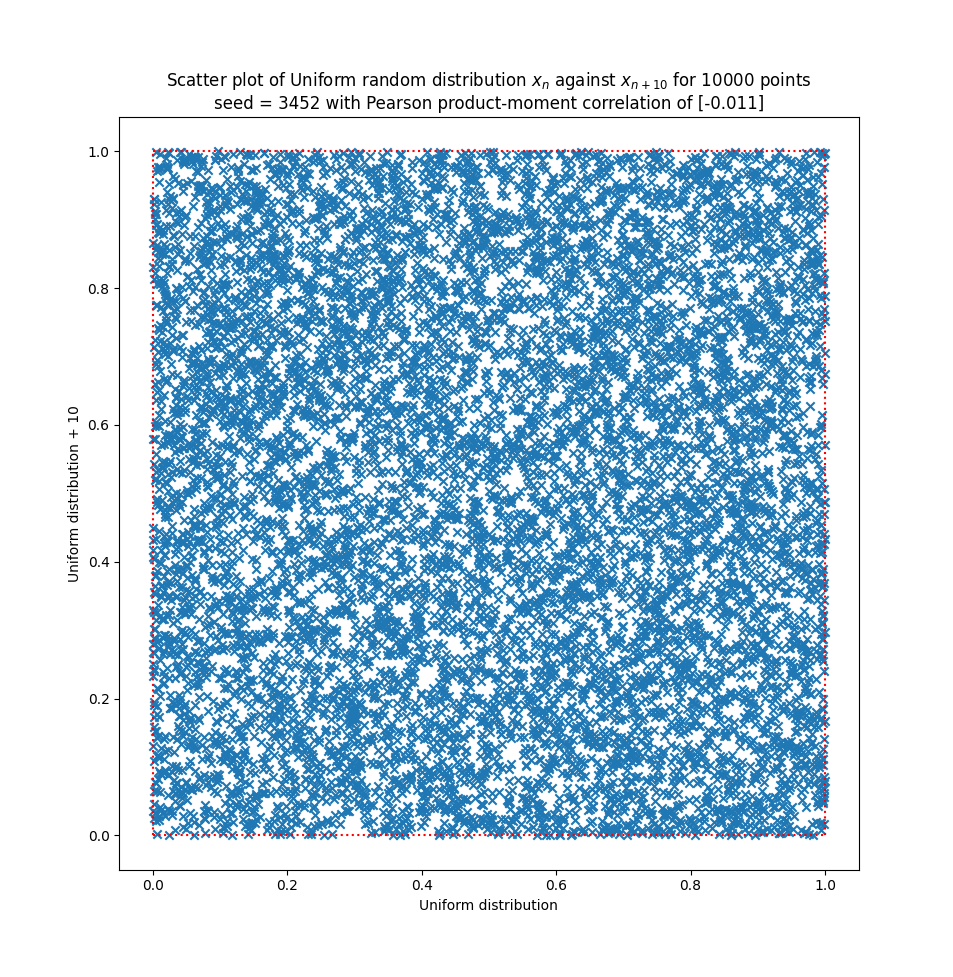
\includegraphics[scale=0.35]{Task_1_Scatter}
    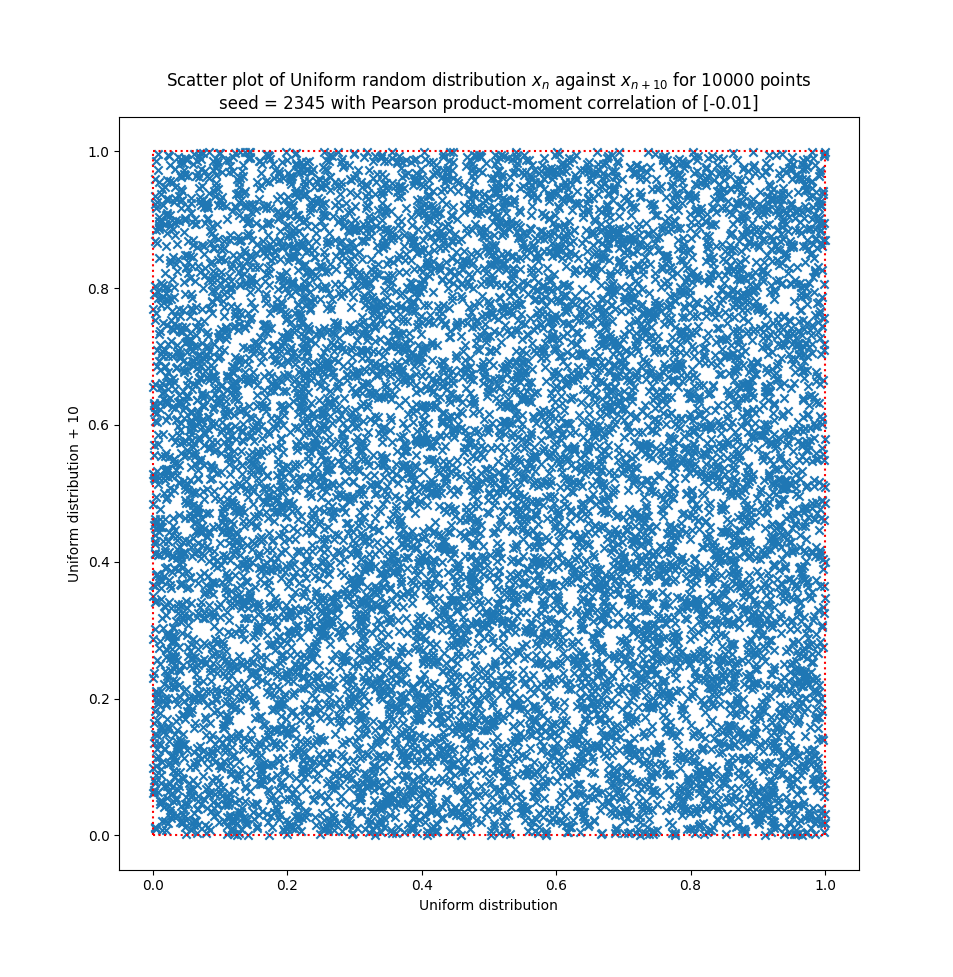
\includegraphics[scale=0.35]{Task_1_Scatter1}
    \caption{"Two scatter plots of 10000 points"}\label{fig1}
\end{figure}


\section*{\underline{Task 2}}
\textbf{Task From Lab Sheet:} \\ \\ Write a program to simulate a partitioned box containing N particles, initially all on one side of the partition, with an equal probability of any one particle moving from one side of the partition to the other in unit time. Present your results graphically as well as textually.
\vspace{1.5em}\\
\textbf{My Result:} \\ \\ The results from figure \ref{fig2} show, at least for the boxes with reasonable particle numbers, a clear trend of the system tending towards equilibrium with mild fluctuations. 
The observation of N $\rightarrow\infty$ shows that the system is following the statistical error of $\frac{1}{\sqrt{N}}$ but the last graph also shows what you'd generally expect a graph of diffusion to look like since, $\Phi_{net}\propto\frac{dn}{dx}$ (Fick's first law), net flux is proportional to the density gradient. 
The speed of diffusion can't be seen graphically since only one transition happens per time step, but as N $\rightarrow\infty$ the gradient would grow $\frac{dn}{dx}\rightarrow\infty$ as $\frac{dn}{dx}=\frac{N-0}{1 (unit box)}$.

\begin{figure}[h]
  \centering
    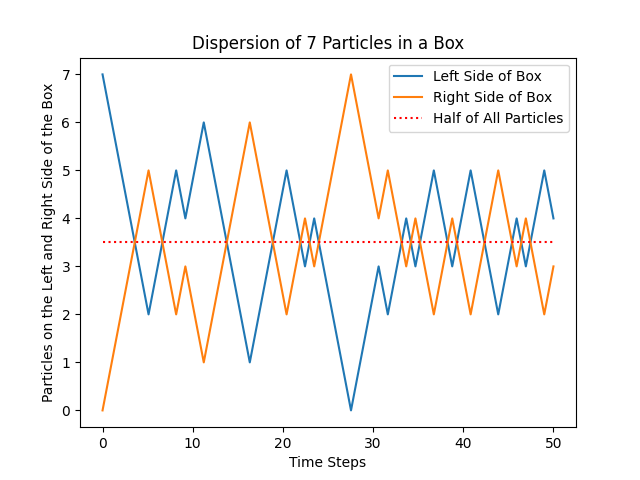
\includegraphics[scale=0.50]{Task_2_Line_7}
    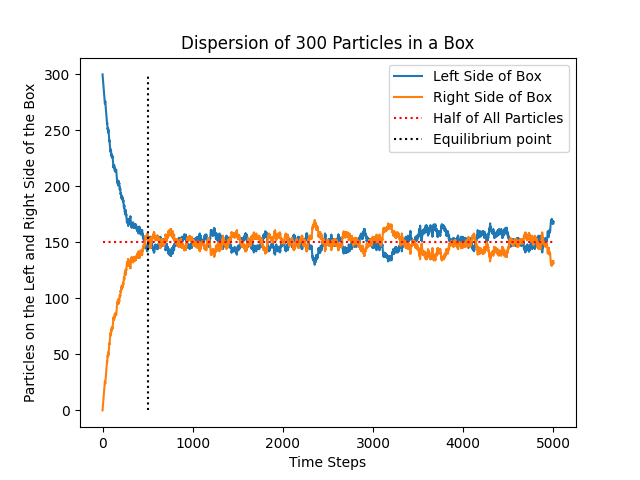
\includegraphics[scale=0.50]{Task_2_Line}
    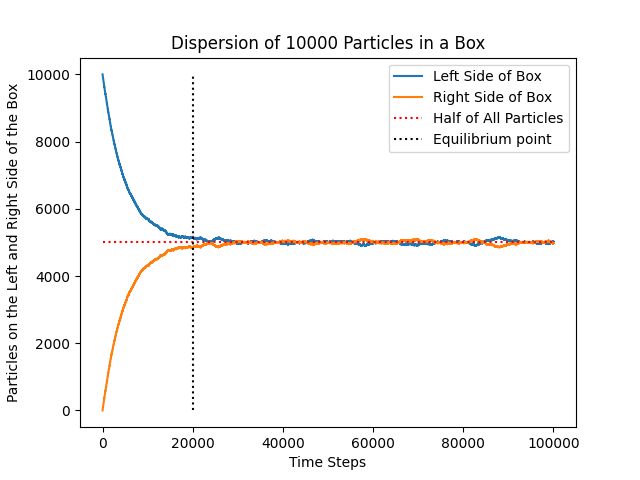
\includegraphics[scale=0.50]{Task_2_Line_10000}
    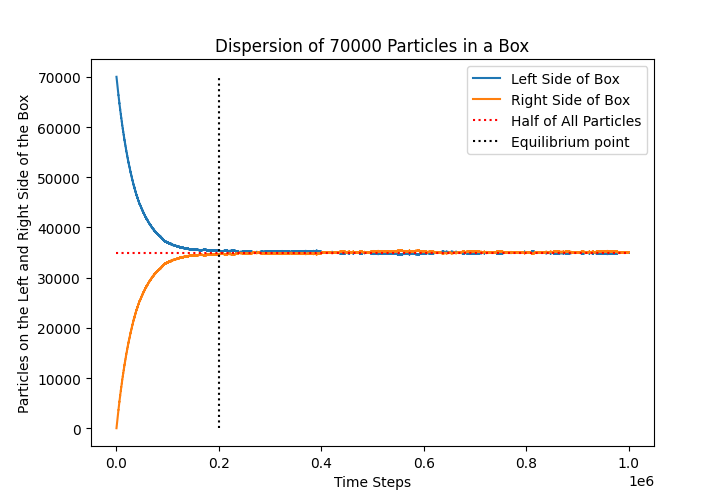
\includegraphics[scale=0.50]{Task_2_Line_70000}
    \caption{"Four plots of the dispersion of particles in a 50/50 split box"}\label{fig2}
\end{figure}


\section*{\underline{Task 3}}
\textbf{Task From Lab Sheet:} \\ \\ Test any properties you calculate in task 2 using sequences from both random number generators in task 1. Discuss whether your results are compatible.
\vspace{1.5em}\\
\textbf{My Result:} \\ \\ In task 2 I used the \href{https://numpy.org/doc/stable/reference/random/generated/numpy.random.randint.html}{numpy.random.randint} and logged the generator that was used to decide which particle got swapped in an array, I then offset the array again, scatter plotted it \ref{fig3} and used \href{"https://numpy.org/doc/stable/reference/generated/numpy.corrcoef.html"}{np.corrcoef} to ensure the random generator is working properly.
\begin{figure}[h]
  \begin{center}
    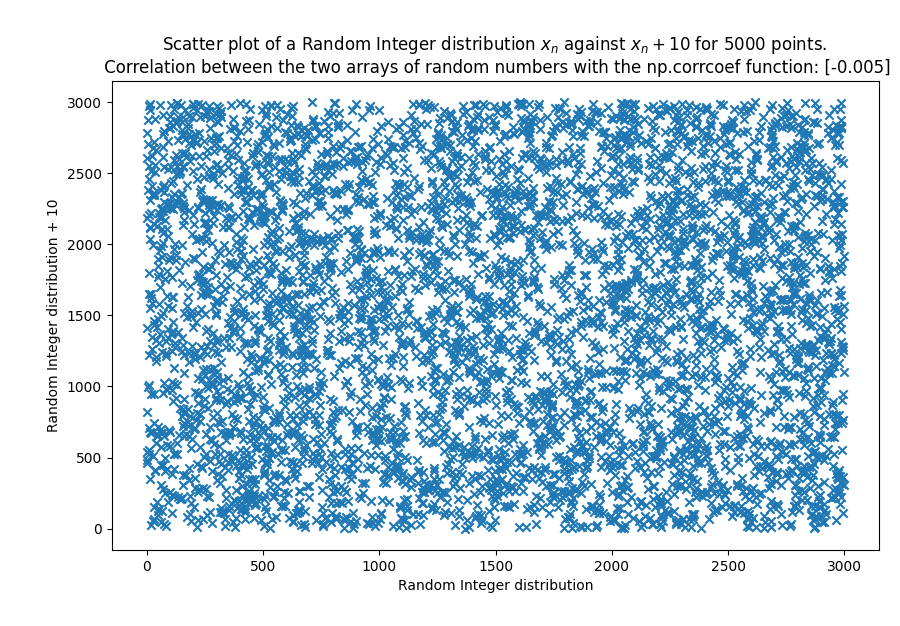
\includegraphics[width=0.75\textwidth]{Task_2_Scatter}
  \end{center}
  \caption{"Scatter plot of the Task 2 data"}
  \label{fig3}
\end{figure}


\section*{\underline{Task 4}}

\textbf{Task From Lab Sheet:} \\ \\ Change the probability so that there is, say, a 75\% chance of any particle from one side of the partition travelling to the other, but only a 25\% chance of any particle going the other way. Discuss your findings and provide numerical evidence if possible.
\vspace{1.5em}\\
\textbf{My Result:} \\ \\ In figure \ref{fig4} it can be seen that after sufficient time either side settles down on a roughly fixed number of particles, $\frac{3}{4}$ and $\frac{1}{4}$. 
This answer makes sense as this experiment is analogous to Osmosis or Osmotic pressure, so since the semi-permeable membrane only lets through a certain number/size of particles and since all else is equal, like volume and temperature, there must be a particle number difference. 
Once again it can be seen that the statistical error, $\frac{1}{\sqrt{N}}$, is inversely proportional to the number of particles in the simulation.
\begin{figure}[h]
  \begin{center}
    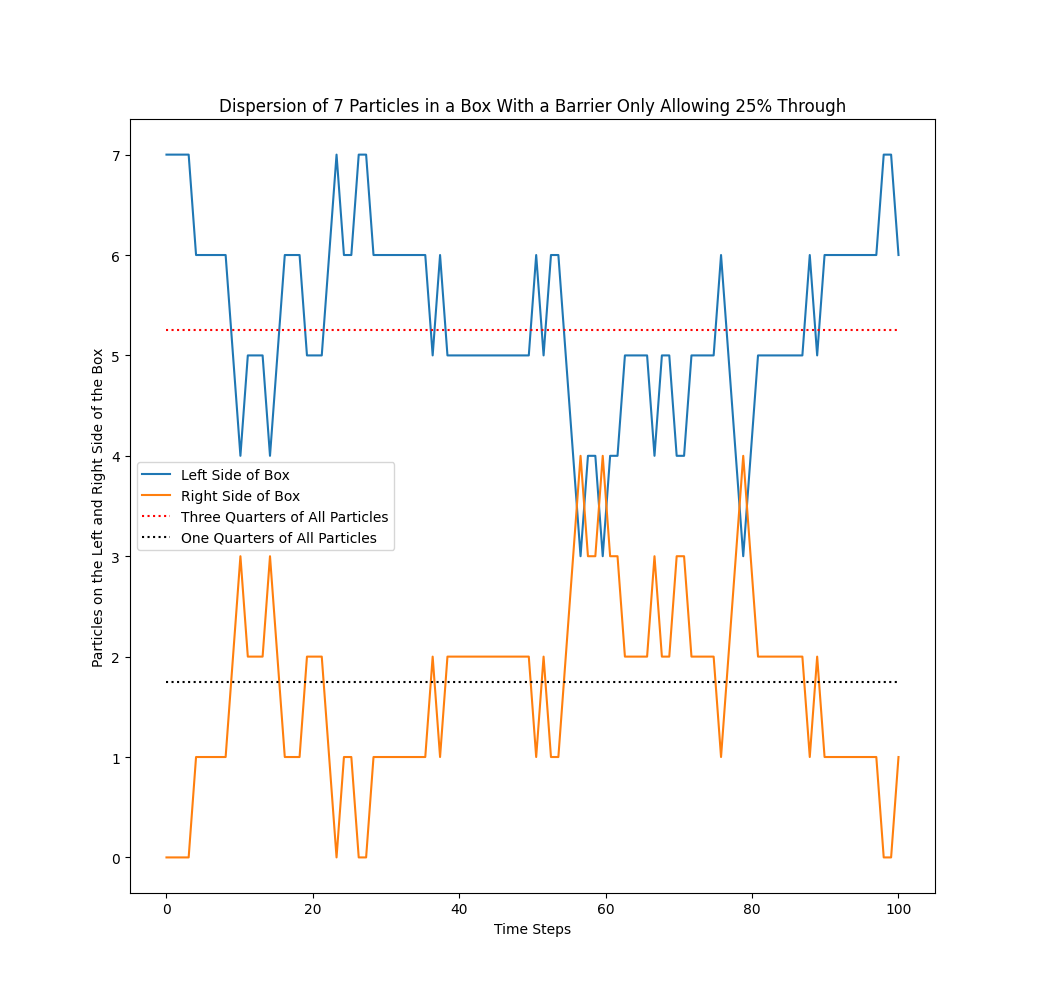
\includegraphics[scale=0.35]{Task_4_Line_7}
    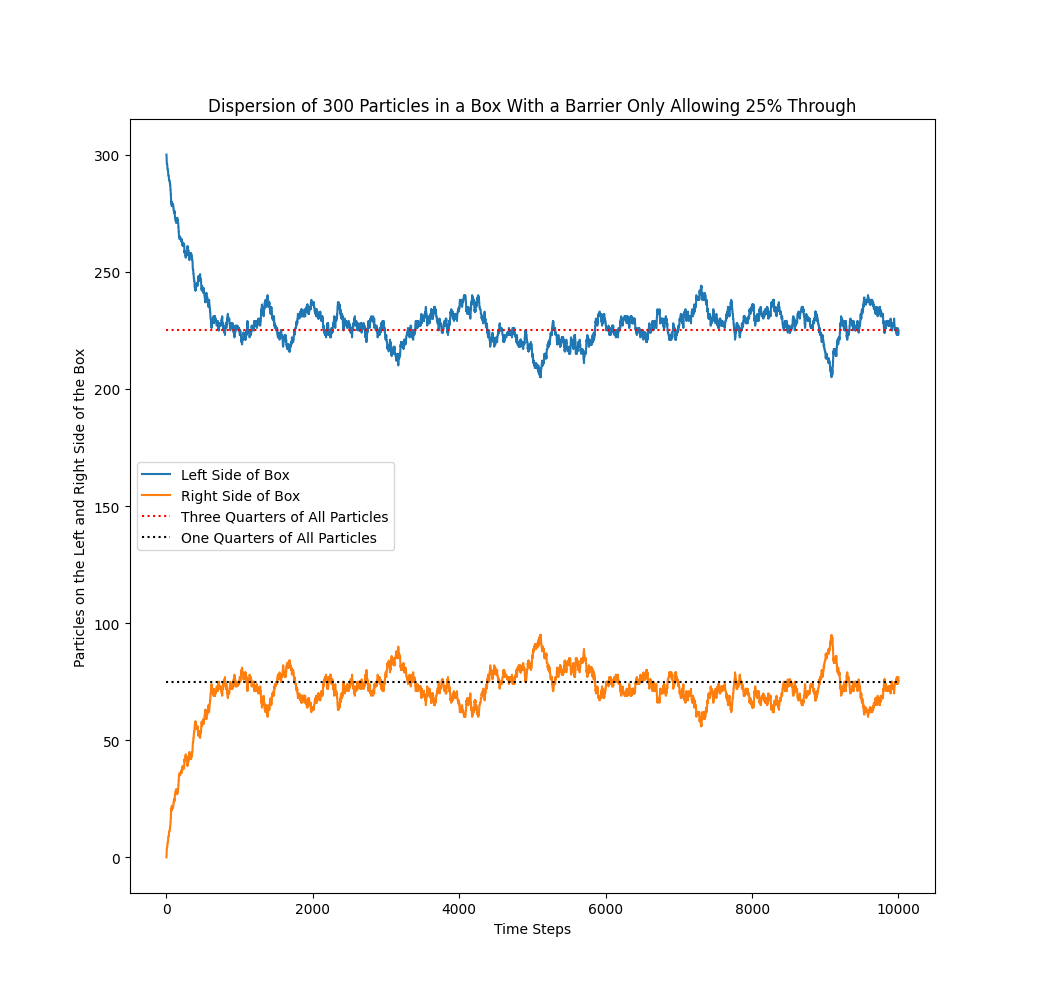
\includegraphics[scale=0.35]{Task_4_Line_300}
    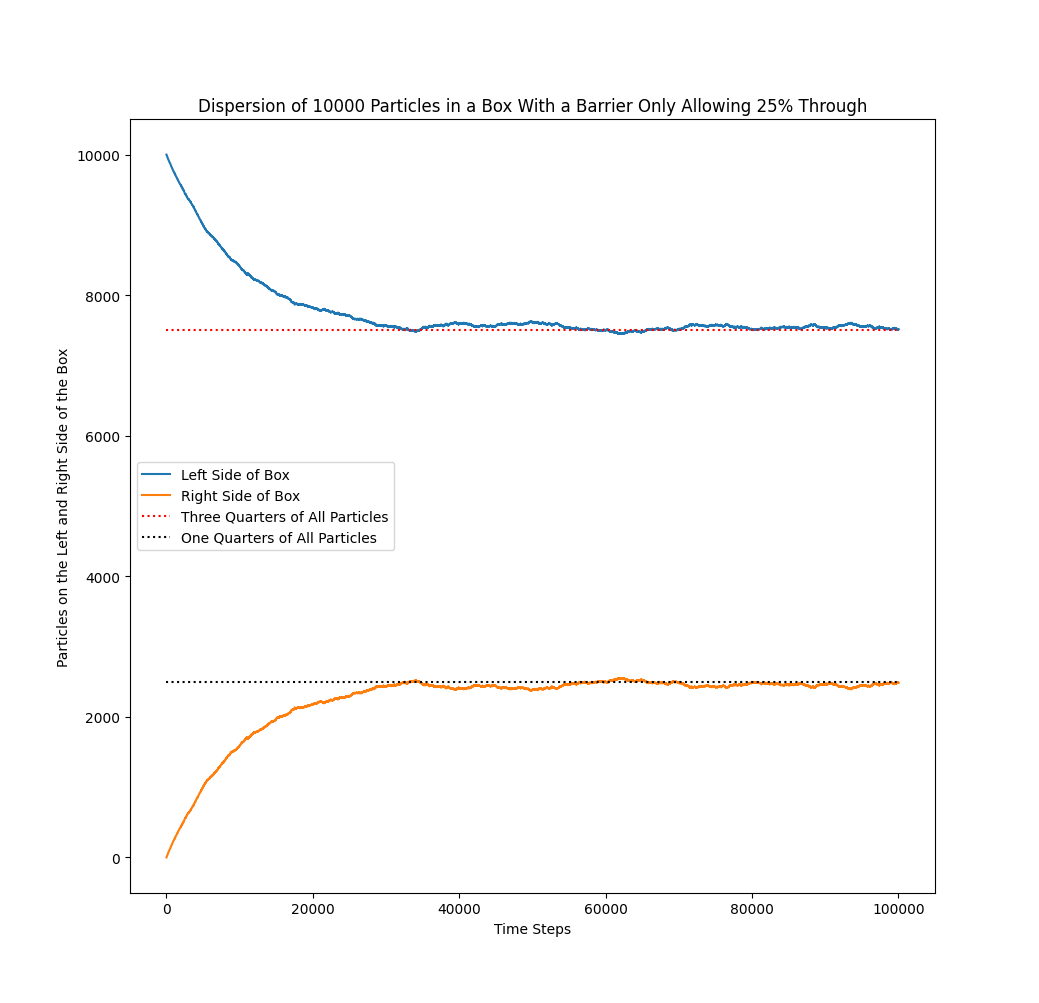
\includegraphics[scale=0.35]{Task_4_Line}
    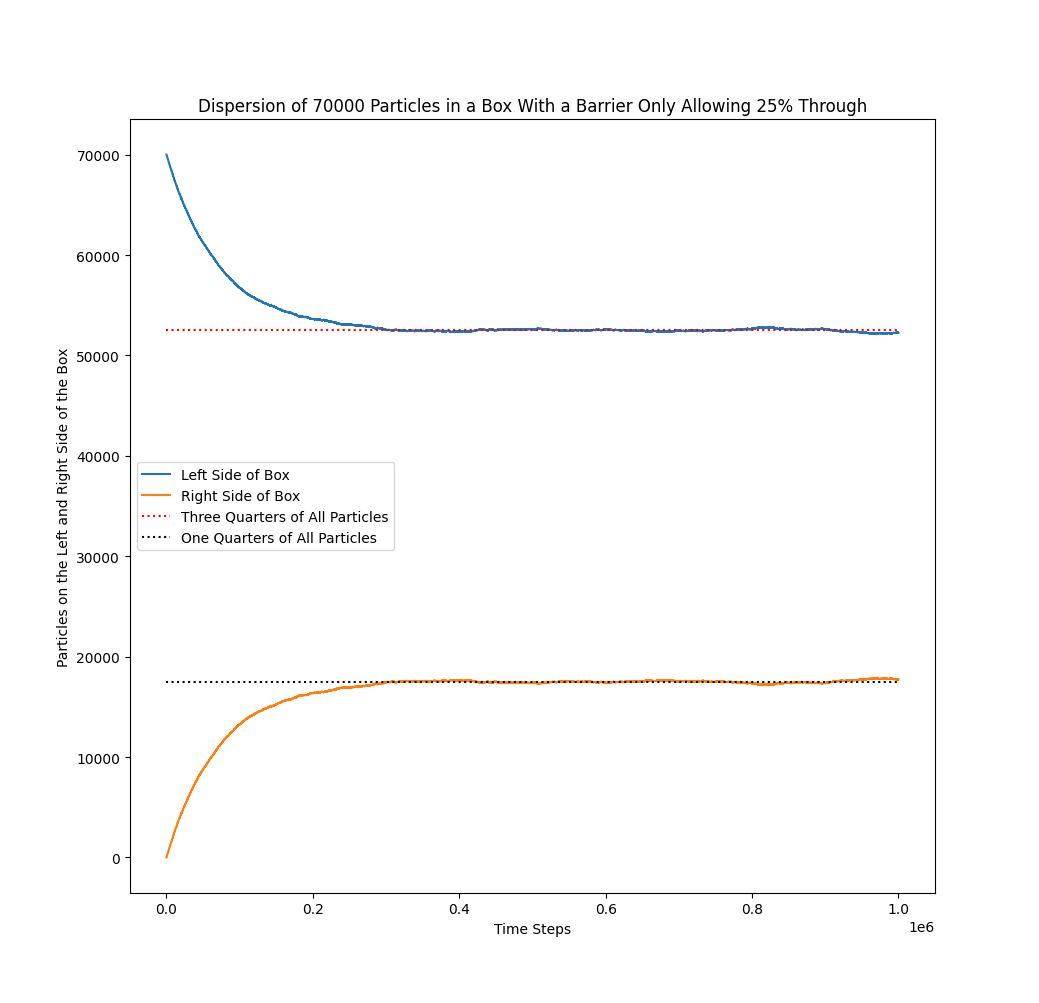
\includegraphics[scale=0.35]{Task_4_Line_70000}
  \end{center}
  \caption{"Four plots of the dispersion of particles in a 25/75 split box"}
  \label{fig4}
\end{figure}

\end{document}
